%
%===============>>  Сторожук Модуль 5 <<=============
%
\setmodule{5}

%BEGIN_FOLD % ====>>_____ Занятие 1 _____<<====
\begin{class}[number=1]
	
	\begin{listofex}
		\item Вычислить: \( 10\cdot\left( \mfrac{3}{2}{15}-\mfrac{2}{5}{18} \right)+12\cdot\left( \mfrac{1}{5}{6}+\mfrac{5}{3}{4} \right) \)
		\item Вычислить: \( (8,94+9,39):(7,57-1,4\cdot2,05) \)
		\item Решить уравнение: \( (x+2,3)\cdot0,2=0,7 \)
		\item Решить пропорцию: \( \dfrac{1,9\cdot0,85}{2,5\cdot0,08}=\dfrac{0,38\cdot3,4}{x} \)
		\item Решить пропорцию: \( \dfrac{1,6\cdot1,7}{x\cdot2,9}=\dfrac{0,051}{0,87} \)
		\item Вычислить:
		\begin{tasks}(1)
			\task \( -\mfrac{1}{5}{11}-\left( -\mfrac{2}{3}{22} \right) \)
			\task \( -3,8-\left( -\mfrac{3}{4}{5} \right) \)
			\task \( -18,31-6,27+(-8,44)-(-31,67) \)
		\end{tasks}
		\item Вычислить:
		\begin{tasks}(3)
			\task \( 2^5+3^4 \)
			\task \( 5^4:5^2 \)
			\task \( \dfrac{2^9}{2^3\cdot2^4} \)
			\task \( \dfrac{6^3\cdot5^2}{3^3\cdot2^4} \)
			\task \( 1,5^4:3^3 \)
			\task \( 8^{-2}\cdot4^3 \)
		\end{tasks}
	\end{listofex}
\end{class}
%END_FOLD

%BEGIN_FOLD % ====>>_____ Занятие 2 _____<<====
\begin{class}[number=2]
	\begin{listofex}
		\item Занятие 2
	\end{listofex}
\end{class}
%END_FOLD

%BEGIN_FOLD % ====>>_ Домашняя работа 1 _<<====
\begin{homework}[number=1]
	\begin{listofex}
		\item  Найти значения выражения:
		\begin{tasks}(2)
			\task \( 2^{\log_26-3} \)
			\task \( 7\cdot5^{\log_54} \)
			\task \( 6^{5\log_63} \)
			\task \( \log_2112-\log_27 \)
			\task \( \log_340,5+\log_36 \)
			\task \( 6^{3\log_62} \)
			\task \( \dfrac{\log_318}{2+\log_32} \)
			\task \( (\log_381)\cdot(\log_6216) \)
		\end{tasks}
		\item 	
			\begin{minipage}[t]{\bodywidth}
			На рисунке изображён график функции \[ f(x)=kx+b. \] Найдите \(f(-200)\).
		\end{minipage}
		\hspace{0.02\linewidth}
		\begin{minipage}[t]{\picwidth}
			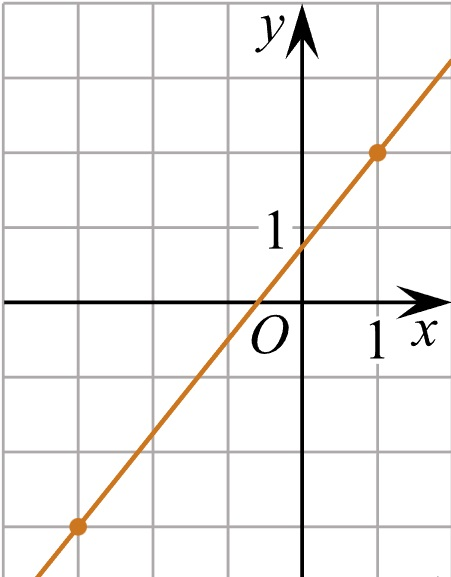
\includegraphics[align=t, width=\linewidth]{../../pics/G101M4C4-1}
		\end{minipage}
		\item 
		\begin{minipage}[t]{\bodywidth}
			На рисунке изображены графики функций \( f(x)=4x^2-25x+41 \) и \( g(x)=ax^2+bx+c \), которые пересекаются в точках \(A\) и \(B\). Найдите абсциссу  \( B \).
		\end{minipage}
		\begin{minipage}[t]{\picwidth}
			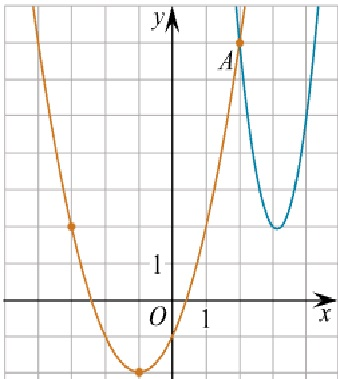
\includegraphics[align=t, width=\linewidth]{../../pics/G111M3PP-1}
		\end{minipage}
	\end{listofex}
\end{homework}
%END_FOLD

%BEGIN_FOLD % ====>>_____ Занятие 3 _____<<====
\begin{class}[number=3]
	\begin{listofex}
		\item Занятие 3
	\end{listofex}
\end{class}
%END_FOLD

%BEGIN_FOLD % ====>>_____ Занятие 4 _____<<====
\begin{class}[number=4]
	\begin{listofex}
		\item Занятие 4
	\end{listofex}
\end{class}
%END_FOLD

%BEGIN_FOLD % ====>>_ Домашняя работа 2 _<<====
\begin{homework}[number=2]
	\begin{listofex}
		\item Найдите значение выражения: \(\dfrac{a(b-3a)^2}{3a^2-ab}-3a\) при \(a=2,18, b=-5,6\)
		\item Упростите выражение: \(\dfrac{6c-c^2}{1-c}:\dfrac{c^2}{1-c}\) и найдите его значение при \(c=1,2\)
		\item Упростите выражение: \(\dfrac{xy+y^2}{15x}\cdot \dfrac{3x}{x+y}\) и найдите его значение при \(x=18, y=7,5\)
		\item Упростите выражение: \(\left(\dfrac{b}{a}-\dfrac{a}{b}\right) \cdot \dfrac{1}{b+a}\) и найдите его значение при \(a=1, b=\dfrac{1}{3}\)
		\item Найдите значение выражения: \(\left(a+\dfrac{1}{a}+2\right) \cdot \dfrac{1}{a+1}\) при \(a=-5\)
		\item Найдите значение выражения: \( (x-3):\dfrac{x^2-6x+9}{x+3} \) при \(x=-21\)
		\item \((a^3-25a) \cdot \left( \dfrac{1}{a+5} - \dfrac{1}{a-5} \right)\) при \(a=-39\)
		\item Запишите десятичную дробь, равную сумме: \( 7 \cdot 10^{-2} + 7 \cdot 10^{-3} + 8 \cdot 10^{-4}\)
		\item Найдите значение выражения:
		\begin{tasks}
			\task \( a^{12} \cdot (a^{-4})^4 \), при \(a = -\dfrac{1}{2}\)
			\task \(\dfrac{(a^7)^3}{a^{18}}\), при \(a=2\)
			\task \( \dfrac{a^9 \cdot a^{12}}{a^{18}} \), при \(a=4\)
		\end{tasks}
		\item Какое из данных ниже чисел является значением выражения \(2^{12} \cdot (2^3)^{-5}\)?
		\begin{tasks}(4)
			\task \(8\)
			\task \(1024\)
			\task \(-8\)
			\task \(\dfrac{1}{8}\)
		\end{tasks}
		\item Найдите значение выражения:
		\begin{tasks}(3)
			\task \( (6 \cdot 10^2)^2 \cdot (14 \cdot 10^{-2}) \)
			\task \( \dfrac{3^5}{27} \)
			\task \( \dfrac{1}{8^{-7}} \cdot \dfrac{1}{8^6} \)
		\end{tasks}
	\end{listofex}
\end{homework}
%END_FOLD

%BEGIN_FOLD % ====>>_____ Занятие 5 _____<<====
\begin{class}[number=5]
	\begin{listofex}
		\item Занятие 5
	\end{listofex}
\end{class}
%END_FOLD

%BEGIN_FOLD % ====>>_____ Занятие 6 _____<<====
\begin{class}[number=6]
	\begin{listofex}
		\item Занятие 6
	\end{listofex}
\end{class}
%END_FOLD

%BEGIN_FOLD % ====>>_ Домашняя работа 3 _<<====
\begin{homework}[number=3]
	\begin{listofex}
		\item ДЗ 3
	\end{listofex}
\end{homework}
%END_FOLD

%BEGIN_FOLD % ====>>_____ Занятие 7 _____<<====
\begin{class}[number=7]
	\begin{listofex}
		\item Занятие 7
	\end{listofex}
\end{class}
%END_FOLD

%BEGIN_FOLD % ====>>_ Проверочная работа _<<====
\begin{exam}
	\begin{listofex}
		\item Проверочная работа
	\end{listofex}
\end{exam}
%END_FOLD